\title{Semantics of Functional Programming}
\subtitle{Formalising PCF in Dependent Type Theory} 
\author[L.-T. Chen]{Chen, Liang-Ting\\
  \href{mailto:lxc@iis.sinica.edu.tw}{\texttt{lxc@iis.sinica.edu.tw}}}
\institute[IIS, Sinica]{Institute of Information Science, Academia Sinica}
\begin{document}
\frame{\maketitle}

\begin{frame}{Formalising \PCF}
  Terms, types, and lists are introduced as (non-dependent) types.
  For example,
  the type for \PCF{} types are introduced as:
  \begin{itemize}
    \item Formation: 
      \[
        \AXC{}
        \UIC{$\Gamma \vdash \mathtt{Type} : \mathcal{U}$}
        \DP
      \]
    \item Introduction:
      \[
        \AXC{}
        \UIC{$\Gamma \vdash \nat : \mathtt{Type}$}
        \DP
        \qquad
        \AXC{$\Gamma \vdash \tau_1 : \mathtt{Type}$}
        \AXC{$\Gamma \vdash \tau_2 : \mathtt{Type}$}
        \BIC{$\Gamma \vdash \tau_1 \Rightarrow \tau_2 : \mathtt{Type}$}
        \DP
      \]
  \end{itemize}

  ~\\
  \textbf{Exercise}. Define types $\mathtt{Term}, \texttt{Type}, \texttt{Cxt}$
  for \PCF{} terms, \PCF{} types, and contexts respectively in \textbf{Agda}.
\end{frame}

\begin{frame}{Predicates}
  In case that you have been polluted by set theory, we distinguish a few
  \alert{set-theoretic} and \alert{type-theoretic} notions. 
  \begin{block}{In set Theory}
    A \textbf{predicate} $P$ over a set $X$ is a subset $P \subseteq X$. 
  \end{block}
  \begin{block}{In type Theory}
    A \textbf{predicate} $P$ over a type $A$ is a judgement 
    \[
      \Gamma \vdash P : A \to \mathcal{U}
    \]
    A \textbf{decidable predicate} over a type $A$ is a judgement
    \[
      \Gamma \vdash t : A \to \top + \top
    \]
  \end{block}
\end{frame}

\begin{frame}{An example of predicates} 
  In set theory, an \textbf{even number} $n$ is commonly defined as a natural
  number satisfying $n = 2 k$ for some natural number $k$, i.e.\ 
  \[
    E_\mathbb{N} = \set{ n \in \mathbb{N}}{ \exists k \in \mathbb{N}.\,
      n = 2k}.
  \]
  ~\\
  In type theory, it is a predicate $\mathtt{even}: \mathbb{N} \to \mathcal{U}$
  introduced by
  \begin{itemize}
    \item Formation:
      \[
        \AXC{}
        \UIC{$\Gamma \vdash \mathbf{even} : \mathbb{N} \to \mathcal{U}$}
        \DP
      \]
    \item Introduction:
      \[
        \AXC{}
        \UIC{$\Gamma \vdash \texttt{zero} : \mathbf{even}\;\mathtt{zero}$}
        \DP
        \qquad
        \AXC{$\Gamma \vdash p : \mathtt{even}\;n$}
        \UIC{$\Gamma \vdash \mathtt{suc}\;p : \mathbf{even}\;(\suc\;(\suc\;n))$}
        \DP
      \]
  \end{itemize}
  where the elimination rule and the computational rule are omitted. 
  \\~\\
  \textbf{Exercise}. Define \textbf{Val} for values of \PCF{} terms.
\end{frame}

\begin{frame}{Set-theoretic relations}
  A \textbf{relation} over a set $X$ is a subset $R \subseteq X
  \times X$, and $(x_1, x_2) \in R$ is written as 
  \[
    x_1 \mathrel{R} x_2.
  \]
  A relation $R \subseteq X \times X$ is 
  \begin{itemize}
    \item \textbf{reflexive} if $x \mathrel{R} x$ for every $x \in X$.
    \item \textbf{transitive} if $x \mathrel{R} z$ whenever $x \mathrel{R} y$
      and $x \mathrel{R} z$
  \end{itemize}
  ~\\
  A \textbf{reflexive transitive closure} of a relation $R$ is
  the smallest reflexive transitive relation $R^*$ containing $R$:
  \[
    R^* \defeq \bigcap \set{ S \subseteq X \times X}
    { R \subseteq S \;\;\text{and $S$ is reflexive and transitive}}
  \]
\end{frame}

\begin{frame}{Type-theoretic relations}
  A \textbf{relation} over a type (set) $A$ is a judgement
  \[
    \Gamma \vdash R : A \to A \to \mathcal{U}.
  \]
  A relation is
  \begin{itemize}
    \item $\textbf{reflexive}$ if
      \[
        \prod[ x : A ]\; R\;x\;x 
      \]
      is provable.
    \item $\textbf{transitive}$ if 
      \[
        \prod[ x : A]\; \prod[ y : A]\;\prod[ z : A]\;R\;x\;y \to R\;y\;z\to
        R\;x\;z
      \]
      is provable.
  \end{itemize} 
\end{frame}

\begin{frame}
  A \textbf{transitive reflexive closure} $R^*$ of a relation $R$ over $A$:
  \begin{itemize}
    \item Formation:
      \[
        \AXC{$\Gamma \vdash A : \mathcal{U}$}
        \AXC{$\Gamma \vdash R : A \to A \to \mathcal{U}$}
        \BIC{$\Gamma \vdash R^* : A \to A \to \mathcal{U}$}
        \DP
      \]
    \item Introduction:
      \[
        \AXC{$\Gamma \vdash x : A$}
        \UIC{$\Gamma \vdash \mathtt{refl}_x : R^*\;x\;x$}
        \DP
      \]
      \[
        \AXC{\begin{tabular}{l}
            $\Gamma \vdash x : A$ \\
            $\Gamma \vdash y : A$ \\
            $\Gamma \vdash z : A$ \\
          \end{tabular}}
        \AXC{$\Gamma \vdash t : R\;x\;y$}
        \AXC{$\Gamma \vdash u : R^*\;y\;z$}
        \TIC{$\Gamma \vdash \mathtt{trans}\;t\;u : R^*\;x\;z$}
        \DP
      \]
  \end{itemize}
  where the elimination rule and the computation rule are omitted.
  \\~\\
  \textbf{Exercise}.
  Show the following statements in \texttt{Transitive-Closure.agda}.
  \begin{enumerate}
    \item $R^*$ is reflexive and transitive for every relation $R$ over $A$.
    \item $R^*$ is the ``smallest'' transitive reflexive relation containing
      $R$.
  \end{enumerate}
\end{frame}

\begin{frame}{Judgements in type theory}
  A \textbf{judgement} is a ternary predicate 
  \[
    {\text{\_}\vdash\text{\_}:\text{\_}} : \mathtt{Cxt} \to
    \mathtt{Term} \to \mathtt{Type} \to \mathcal{U}.
  \]
  in type theory. 
  \\~\\
  The introduction rule for $\suc$ in \PCF{} is formalised as
  \begin{center}
    \only<presentation>{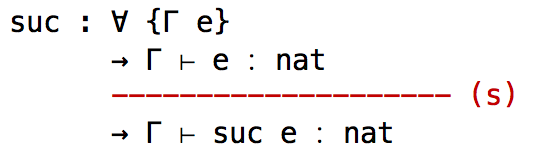
\includegraphics[scale=.5]{suc.png}}
  \end{center}
  \textbf{Exercise}. Define a type of the typing rules of \PCF.
\end{frame}

\begin{frame}{Progress Theorem in type theory}
  Recall Progress Theorem:
  \begin{theorem}
    Every closed well-typed \PCF{} term $\M$ is either a value or there exists
    another term $\M'$ such that $\M \leadsto \M'$. 
  \end{theorem} 
  which corresponds to a witness of 
  \begin{align*}
    & \prod[ \M : \texttt{Term}]\prod[ \tau : \texttt{Type} ] \\
    & [\,] \vdash \M : \tau \to (\mathtt{Val}\;\M) +
    \Sigma[ \M' : \mathtt{Term} ]\;
    \M \leadsto \M'
  \end{align*}

  \textbf{Exercise}. Finish \texttt{PCF\_blank.agda}. 
\end{frame}
\end{document}
